\documentclass[10pt,twocolumn,letterpaper]{article}

\usepackage{cvpr}
\usepackage{times}
\usepackage{epsfig}
\usepackage{graphicx}
\usepackage{amsmath}
\usepackage{amssymb}
\usepackage{graphicx}


% Include other packages here, before hyperref.

% If you comment hyperref and then uncomment it, you should delete
% egpaper.aux before re-running latex.  (Or just hit 'q' on the first latex
% run, let it finish, and you should be clear).
\usepackage[breaklinks=true,bookmarks=false]{hyperref}

\cvprfinalcopy % *** Uncomment this line for the final submission

\def\cvprPaperID{****} % *** Enter the CVPR Paper ID here
\def\httilde{\mbox{\tt\raisebox{-.5ex}{\symbol{126}}}}

% Pages are numbered in submission mode, and unnumbered in camera-ready
%\ifcvprfinal\pagestyle{empty}\fi
\setcounter{page}{1}
\begin{document}

%%%%%%%%% TITLE
\title{Solving the Rubik's Cube without Human Interaction}

\author{Victoria Som de Cerff\\
{\tt\small vs2606@columbia.edu}
% For a paper whose authors are all at the same institution,
% omit the following lines up until the closing ``}''.
% Additional authors and addresses can be added with ``\and'',
% just like the second author.
% To save space, use either the email address or home page, not both
\and
Michael Kovalski\\
{\tt\small mhk2160@columbia.edu}
}

\maketitle
%\thispagestyle{empty}

%%%%%%%%% ABSTRACT
\begin{abstract}
We intend to investigate known methods of solving a Rubik's Cube without the need for human-tuned heuristics and reproduce similar results. 
\end{abstract}

%%%%%%%%% BODY TEXT
\section{Introduction}

A generally intelligent agent must be able to teach itself how to solve problems in complex domains with minimal human supervision.  Developing heuristics has proven to limit the search space for these problems and find good solutions, but may sometimes be too complex to come up with and may not necessarily yield optimal performance. An agent without human interaction would be able to learn promising moves by exploring the search space on it’s own and determine what states are the most optimal to be in. In the work done in “Solving the Rubik’s Cube Without Human Knowledge” they propose a method to solve a self play game without defined heuristics as rewards for intermediate states leading up to the ultimate goal state.  

Their algorithm is able to solve 100\% of randomly scrambled cubes with a scramble distance of 15, while achieving a median solve length of 30 moves. Our goal was to replicate the algorithm used in this paper to solve both 2x2 and 3x3 rubik's cubes without necessarily needing to  search the entire state space of $4.3 x 10^{19}$ possible configurations given a set of computational resources.


%-------------------------------------------------------------------------

%------------------------------------------------------------------------
\section{Related Works and References}

There are previous rule based methods used to solve rubik’s cubes in a number of steps, such as knowing which layers to rotate first and how to rearrange given certain states [1]. However, this requires human intuition up front.  The upper bound was proven on how many steps it takes to solve a rubik’s cube from any starting configuration [2], although there is no simple rule based method to solve this problem. There have been previous attempts to solve this problem computationally. Heuristic based methods have been successful by using a variation of A* [3] which finds the median optimal steps away to be 18 moves. Recently, a DNN was used with featuring engineering to find the optimal route to the solution [4] but these methods take some time to run. Additionally, genetic programming has been used but fail to make optimal decisions when more than 5 steps away from the optimal solution [5]. Recent work has been done to figure out how to solve a rubik’s cube without human interaction by using the Autodidactic Iteration algorithm [6], which is similar to the AlphaZero algorithm [7] which uses Monte Carlo Tree Search to help find solutions. This algorithm can solve the rubik’s cube with 100\% success when moved 15 states away from the solved state, while on average being able to solve these puzzles in 30 steps. However, there is currently no source code for how to implement this solver. In addition, the paper uses 3 GPUs to search through the space and run neural networks for function approximation.

%-------------------------------------------------------------------------

%------------------------------------------------------------------------
\section{Problem Formulation}

We wanted to exactly replicate the work done in “Solving the Rubik’s Cube Without Human Knowledge” and develop a code base to solve rubik's cubes deep within a search tree. In this paper, the goal is to solve the rubik's cube without the use of explicit human tuned heuristics by exploring the search space and letting a neural network be used as a guide to help through the Monte Carlo tree search, similar to the methods used in AlphaZero [7]. As of now, there is no source code available for the paper. A code base needed to be developed to help iterate through the neural network training and Monte Carlo tree search. Code was developed in python and Tensorflow, where a rubik's cube simulator was built to represent the cube in a low dimensional feature space. The neural network was built to replicate the model used in the original paper, with both value and policy output layers. This is a more efficient way to train the network as opposed to having both a value and a policy network.

\subsection{Model Representation}
There are several ways to represent a rubik's cube.  Most simply, a 3x3x3 matrix.  However, since with a rubik's cube we are only concerned with the external faces, that leaves many null extraneous values internal to the matrix.   For that reason we use an alternative approach for laying out the state of our rubiks cube as 20x24 matrix where each value in the matrix has a specific meaning to the current state of the cube and is represented as a sparse matrix.

Consider a solved cube in a fixed orientation.  There are 20 unique positions, 8 corners and 12 edge pieces.  We denote each position by the colors in that position in the fixed solved state.  For each of the 20 positions there are 24 unique color orientations that can be placed in that position.  Our state matrix is a one hot encoding of which color orientation exists each position. 

It is important for the naming convention that we fix primary (top:white / bottom:yellow), secondary (left:blue / right:green) and tertiary front:orange / back:red) planes.  

The 12 edge pieces are WB, WG, WO, WR, YB, YG, YO, YR, GO, GR, BO, BR.  In each of those unique positions, every one of those initial color orderings and their inverse can occur in that position.  i.e. the WB position can have WB, BW, WG, GW, WO, OW, etc.  Hence 24 states for the edges.  

The 8 corner pieces are WOB, WBR, WGO, WRG, YBO, YBR, YRG, YOG.  These positions are uniquely named starting in the dominant plane and reading off the remaining corner colors in a clockwise ordering.  Each color ordering can have three states by performing a clockwise rotation of the corner.  i.e. WOB $\leftarrow$ OWB $\leftarrow$ BOW.  Each corner position can have all 3 states for each of the 8 initial color orderings.  Hence 24 states for the corners. 

Now every entry in the matrix has meaningful information.  cube[position][orientation]=1 if that orientation of colors exists in that position.  Again this is a one hot encoding so only one color orientation can appear in a position at a time. 

When a face is turned the edges and corners not only move positions but will change orientation accordingly.   More details on orientation changes for cube rotations can be found from this source [8].

The simulator maintains the state of the cube using this 20x24 representation and performs the necessary changes when given face to turn.  We have 12 valid moves.  Each of the six faces can either move clockwise or counter clockwise 90 degrees. 

In addition, a 2x2 rubik's cube model was developed to help us iterate more quickly through the design process and given our set of computational resources.  This is a similar representation to a 3x3 rubik's cube, the only difference being that there are no "edge" pieces, only corners.  For a 2x2 rubik's cube, God's number is consider to be 14 in the quarter turn metric (the metric used for this model). Our goal of this was to see if a smaller cube would be easier to train, given the amount of resources used in the original paper were not feasible for our project constraints. 

\section{Design}
As noted above, the goal was to replicate the original paper. To do this, a code base was built using the following structure. We replicated the paper exactly to initially start with a solid foundation on how the problem was solved. There are two main parts of the code base which allowed us to solve a rubik's cube: A neural network to help learn valuable moves and a monte carlo tree search which used this neural network to reduce search.

\section{Training}

\subsection{Architecture}
We used a feed forward neural network as the architecture.  The network takes in a 20x24 matrix for a 3x3 cube  representing the current state of the rubik's cube.  There are then two dense layers, the result of which splits apart to the derive the two outputs: 1 dimensional scalar v, representing the reward value, and a 12 dimensional vector p, representing the probability of selecting each of the possible moves for the next state.  These outputs direct the execution of the Autodidactic Iteration and Monte Carlo Tree Search. The architecture can be seen in Figure 1.

\begin{figure}
  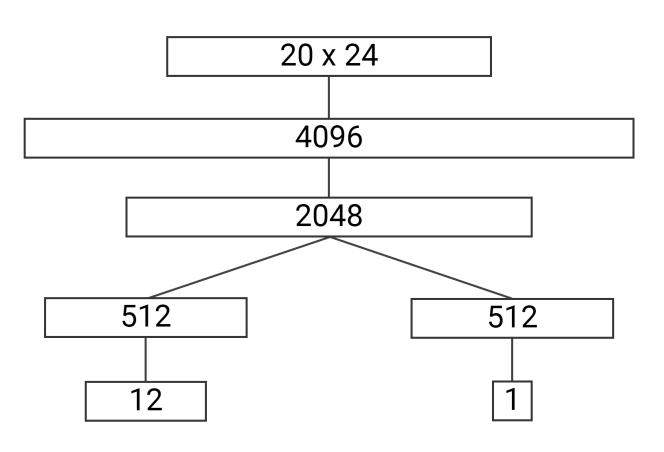
\includegraphics[width=\linewidth]{net.png}
  \caption{Neural network.}
  \label{fig:net}
\end{figure}

\subsection{Autodidactic Iteration}
The goal of autodidactic iteration is to help efficiently guide tree searching by using a neural network to learn a value and policy function to determine which moves are best. We start from a solved state rubik's cube, make $N$ moves from the solved state, and determine a value each cube's children at each of the $N$ states. At each state $n$, we expand the children for that cube and run the children state through a neural network to receive a value approximation. The approximation is then added to the true reward of each child. Finally, a maximum value is determined from the children and the parent cube is trained using the maximum value and reward sum from a child node and the policy that lead to such a value. After seeing these N cubes, the N states, value, and policy combinations were sent to the neural network as a single batch for training.
\\

Formally, the rubik's cube starts from initial solved state $S_0$. The rubik's cube is then moved from the previous state to a new state, which is done $N$ times. From each state $S_n$, $n \in N$, the rubik's cube is then expanded $\forall$ children $s_i$, where $i \ \exists \ [12]$ since there are 12 possible children. $\forall$ children, we run $f_\theta$ on the states $s_i$ to receive a value and policy. The true reward is then added to each of the value approximations made by $f_\theta$. 
The maximum value of $s_i$, $(R(s, a) + \gamma v_i(s_i))$,  is then chosen, and the $argmax \ (R(s, a) + \gamma v_i(s_i)) \forall a \in A$ is chosen as the correct policy. A discount factor $\gamma$ is used to help the learning algorithm understand how future rewards lose value, which additionally proved to be absolutely necessary to keep the training from diverging. $f_\theta$ then does a forward pass using the state $S_n$ as input, and the loss is calculate based on $(R(s, a) + \gamma v_i(s_i))$,and $argmax (R(s, a) + \gamma v_i(s_i))$. This process is completed $M$ times.

In addition, it was noted in the original paper that the value approximations were weighted so that as the rubik's cube moved further away from a solved state, the training weight decreased. This was also implemented in our version and proved to be useful to avoid diverging during training.


\subsection{Methods}
During training, some additional parameters were tweaked that were not mentioned in the paper. During autodidactic iteration, a discount factor was added to the value approximation during each training step to avoid diverging. Initially, our training would diverge without this, as it seemed to get stuck in a value approximation loop from the solved state to a state one away.

Additionally, we started training by first learning cubes that were very close to the solved cube. To do this, we started with moving a single step away from the solved cube and learning on those cubes. After some number of steps, we then expand the learning to also learn cubes at most 2 steps away from the solved state. This seemed to help with convergence, as previously our training took quite some time to reach a reasonable training loss. As the number of steps away from the cube increased, we trained longer on these examples to ensure that it saw plenty of these types of examples during training time. 

Learning rate decay was used to avoid divergence from a true solution. As the method saw more and more cubes at each stage, the training cost seemed to fluctuate around a central value. By implementing learning rate decay, the loss seemed to taper off near the end of training.

Finally, batch sizes were tested to observe differences in training behavior. From our experience, larger batch sizes helped with smoother convergence to a end loss function, but in our case were very expensive and time consuming to use for training. We ended up choosing a batch size somewhere in the middle during training.

\subsection{Innovation}
The initial method uses a non-heuristic based approach to try and solve the rubik's cube. By doing this, human based heuristics are removed and the neural network thus approximates these heuristics for us. 

One thing that was not noted in the paper that we added into our code was ensuring that after a move, the rubik's cube did not make the opposite move afterwards to put it back to a state it had previously seen. For example, turn the top face right followed by turning the top face left would result in a configuration the rubik's cube had seen. The reason for this modification is we wanted to explore as many possible states as possible within the rubik's cube for each batch. By removing duplicate moves, we can ensure that the rubik's cube always has an unseen state during the iteration. However, both options were tested for training and we did not see large results in terms of cost. Because of this, we allowed the algorithm to move back to previous states. More testing could be done with this to observe performance.

While the results using this method has good results in the original paper, an additional goal is to explore the hyperparameter space  and see if there are better combinations that can help to train the neural network more efficiently. Methods such as grid search Bayesian Optimization  will be used to find which hyperparamters lead to the most effective training. These hyperparameters may include layer size, number of layers, activation functions, depth of tree search in ADI, etc. The original paper notes that it uses a search depth of 1, but the code can be easily modified to search deeper into the tree when training the neural network using Autodidactic Iteration. In addition to neural network hyperparameters, the Monte Carlo tree search also has parameters that can be tweaked, such as the exploration and virtual loss, which help with exploring the tree without getting stuck always going down the same branch.

We also scaled the batch size as the training continued. We initially started with a batch size of 5. As we moved further and further away from the solved state, we would increase by another factor of 5, or the original batch size intended. This seemed to be a good trade off in terms of performance and training accuracy.


\section{Inference}

\subsection{Monte Carlo Tree Search}

After the neural network is trained, we use Monte Carlo tree search to look through the space to determine which paths to take to find a solved state, using the neural network $f_\theta$ as a guide as to what paths to take. 

Initially, we start with a random state for the cube $S$. Each node of the search tree has some values assoicated with it, such as the number of times it has chosen action $a$ from state $s$, the maximum value of action $a$ from state $s$, the virtual loss function for each action $a$, and the prior probability of action $a$ from state $s$.

The tree is traversed in the following fashion: An action $a$ is selected at each node by taking the maximum value of $A=argmax_a U_{s_{t}}(a) + Q_{s_{t}}(a) $, where the two values help to explore the tree using factors such as how many times it has been visited, the maximum value of the tree, as well as hyper parameters such as $c$, which is an exploration hyperparameter, and $v$, which discourages the search from taking the same path.

When a leaf node is reached, all children are expanded and initialized, so that $N_i = 0$, $W_i = 0$, $L_i = 0$, and $P_i = p_i(f_\theta (s_i))$. The values is  then backed up all the way to the root node, where $W_s(A_t) = max(W_s(A_t), v_i(A_t)$, $N_i += 1$, $L_s -= v$.

The simulation is completed once a solved state is reached, or a maximum number of iterations are taken.

\subsection{Methods}

\subsection{Innovation}

%-------------------------------------------------------------------------

%------------------------------------------------------------------------
\section{Methodologies and Results}

Initially, we started off with the easier problem of solving a 2x2 rubik's cube. This decision was made as to help us understand how we could go about solving the problem originally without a code base to start with. Additionally, we had computational resource constraints, which we will talk about how these come into play later on.

We started by training a neural network to learn the 2x2 cube value and policy functions. We trained the network with moves up to 20 quarter turns away from the solved state. God's number for the 2x2 cube is 14 in the quarter turn metric, and because we allow the rubik's cube to move to any other state from any state, we felt 20 would sufficiently cover the search space. We trained the network for 2 million iterations. We trained with a batch size starting at 5 and let it grow over time with each move away from the orignal solved state (when we let the rubik's cube go to 2 moves, batch size increased to 10, to 3 it increased to 15, etc.). This decision allowed us to iterate pretty quickly.  We started learning the cube at only 1 step away from the solved state for a fixed number of iterations (we chose 4000). After this, we allowed the cube to move 2 turns past the solved state. We then trained for 8000 iterations, at 3 turns 12000 iterations, so forth. We ran for up to a total of 1 million iterations. After training, we ran MCTS on the solved cubes of varying distances from the origin up to 14 moves away and observed on average what percentage of cubes we were able to solve, how many nodes it needed to explore, and the average number of moves to get to a final solution. We compared this at first with a brute force solution to make sure our neural network was learning something interesting on how to solve. 



\begin{figure}
  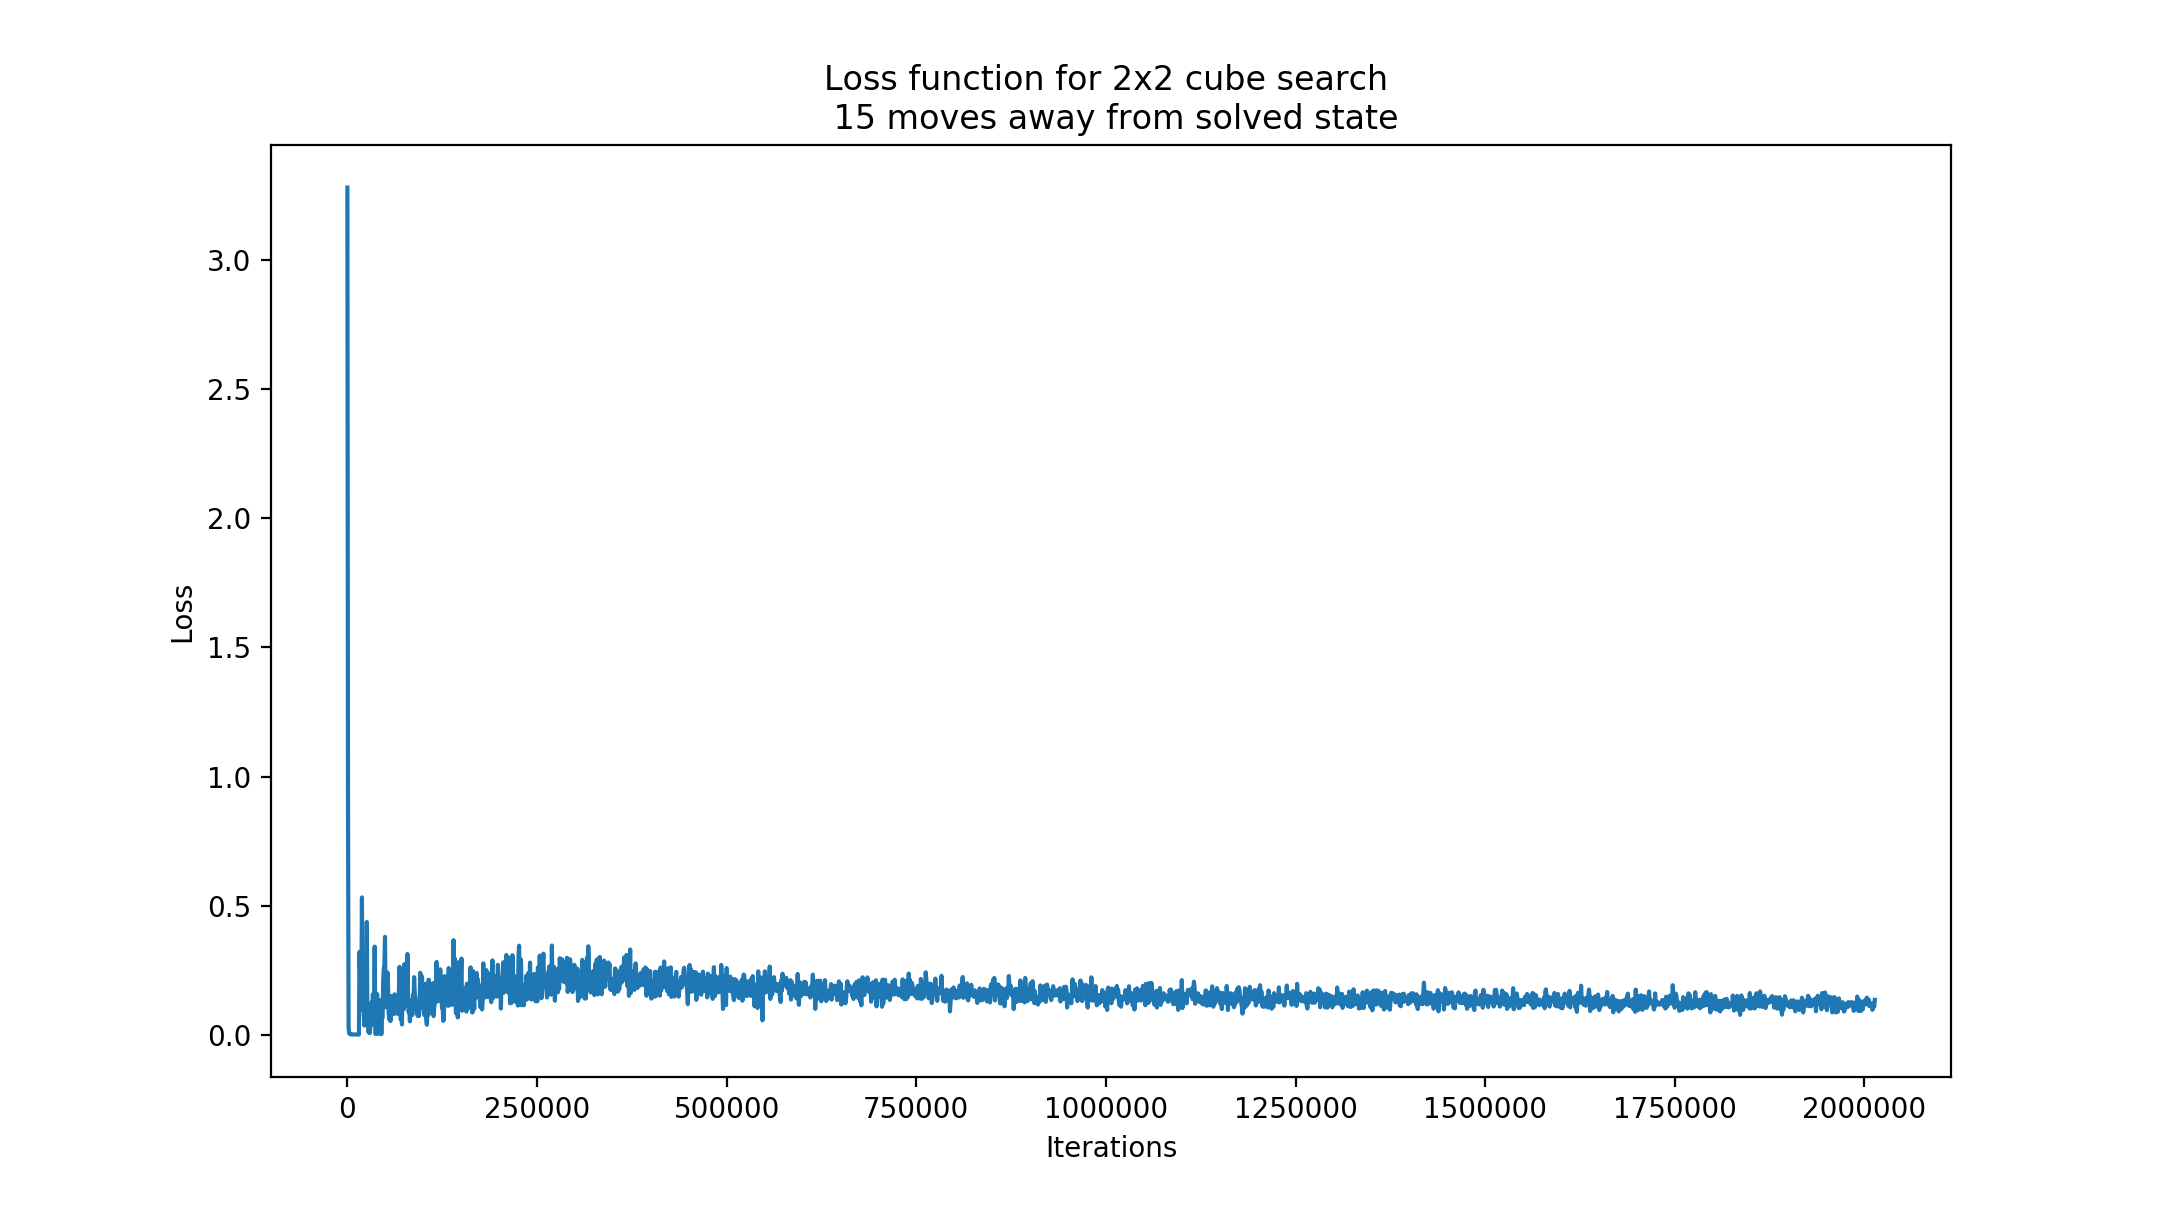
\includegraphics[width=\linewidth]{loss.png}
  \caption{Neural network.}
  \label{fig:net}
\end{figure}

\subsection{Final Comments}

Our initial goals were to solve the 3x3 rubik's cube as done in the paper. However, as training progressed, we started to understand why the computational resources listed were used (32 core machine with 3 GPUs). One thing that we had noticed is that when training, the bottleneck became generating the cubes on the CPU. This performance lead to starving the GPU of training data and leading it idle for much of training time. Our GPU machine used on google cloud had only 2 cores, so we could not push the data generation as far as we would have liked to. More cpus would tremendously speed up our data generation process.

These resources had an impact on the batch size. While we wanted to use a large batch size, as from some experimenting it helped with better convergence, it made training very slow. To generate the amount of data to saturate the GPU memory took a very long time. We ended up choosing a batch size of around 5 for the 2x2 cube to get results quickly, but using multiple GPUs as used in the paper would help us to use a larger batch size. Techniques such as gradients reductions, as used in the horovod framework, could be utilized to achieve smoother gradient decent [9].

%-------------------------------------------------------------------------

%------------------------------------------------------------------------


\section{Code}

While most of the methods and concepts were pulled from the paper "Solving the Rubik’s Cube Without Human Knowledge", there was not an available repository.  The model construction, neural network, and search algorithm all had to be written from scratch.  Our implementation can be found on github here: https://github.com/mkovalski/cs4995\textunderscore cube.  Our network was implemented using the Tensorflow library. 

The code allows users to try different hyperparameters during training, such as batch size, iterations, number of iterations at a certain number of steps away from the cube, etc.   We also allow the user to try out the MCTS algorithm on a trained network. The code let's you train on a 2x2 or a 3x3 rubik's cube. 

%-------------------------------------------------------------------------

%------------------------------------------------------------------------


\begin{thebibliography}{9}

\bibitem{}
https://ruwix.com/the-rubiks-cube/how-to-solve-the-rubiks-cube-beginners-method/

\bibitem{}
https://epubs.siam.org/doi/10.1137/120867366

\bibitem{}
https://www.cs.princeton.edu/courses/archive/fall06/cos402/papers/korfrubik.pdf

\bibitem{}
Robert Brunetto and Otakar Trunda. Deep heuristic-learning in the rubik’s cube domain: an experimental evaluation. 2017.

\bibitem{}
https://dl.acm.org/citation.cfm?id=2908887

\bibitem{1805.07470}
Stephen McAleer, Forest Agostinelli, Alexander Shmakov and Pierre Baldi.
\newblock Solving the Rubik's Cube Without Human Knowledge, 2018;
\newblock arXiv:1805.07470.

\bibitem{1712.01815}
David Silver, Thomas Hubert, Julian Schrittwieser, Ioannis Antonoglou, Matthew Lai, Arthur Guez, Marc Lanctot, Laurent Sifre, Dharshan Kumaran, Thore Graepel, Timothy Lillicrap, Karen Simonyan and Demis Hassabis.
\newblock Mastering Chess and Shogi by Self-Play with a General Reinforcement Learning Algorithm, 2017;
\newblock arXiv:1712.01815.

\bibitem{}
https://www.ryanheise.com/cube/cube\textunderscore laws.html

\bibitem{1802.05799},
Author = {Alexander Sergeev and Mike Del Balso},
Title = {Horovod: fast and easy distributed deep learning in TensorFlow},
Year = {2018},
Eprint = {arXiv:1802.05799}

\end{thebibliography}

{\small
\bibliographystyle{ieee}
\bibliography{egbib}
}

\end{document}
